\documentclass[a4paper]{article}

\usepackage[utf8]{inputenc}
\usepackage{erk}
\usepackage{times}
\usepackage{graphicx}
\usepackage[top=22.5mm, bottom=22.5mm, left=22.5mm, right=22.5mm]{geometry}

\usepackage[slovene,english]{babel}
\usepackage{hyperref}
\usepackage{url}

\let\oldfootnotesize\footnotesize
\renewcommand*{\footnotesize}{\oldfootnotesize\scriptsize}

\begin{document}
\title{Nevarna voznja}

\author{Gašper Smerkolj$^{1}$, Gregor Berger$^{2}$} % use ^1, ^2 for author(s) from different institutions

\affiliation{	$^{1}$Univerza v Ljubljani, Fakulteta za računalništvo in informatiko \\ 
				$^{2}$Univerza v Ljubljani, Fakulteta za računalništvo in informatiko }

\email{E-pošta: gs3493@student.uni-lj.si}

\maketitle

\selectlanguage{slovene}

\begin{abstract}{Abstract}
Pri izdelavi igre za seminarsko nalogo pri računalniški grafiki imava namen uporabiti okolje WebGl ter programski jezik Javascript. Igra bo zabavala igralca z samo težavnostjo vožnje avtomobila mimo ovir ter z zbiranjem kovancev katere bo igralec lahko uporabil. Če bo imel dovolj zbranih kovancev bo namreč lahko zapeljal čez ovire, če pa zapelje preko ovire brez zadostnega števila za določeno oviro se gre igralec na začetek igre. Vsaka različna ovira bo
ob trku odvzela določena števila kovancev. Dlje časa kot traja 1 igra težje postaja izogibanje ovir.
\end{abstract}


\section{Pregled igre}
\begin{figure}[!htb]
	\begin{center}
		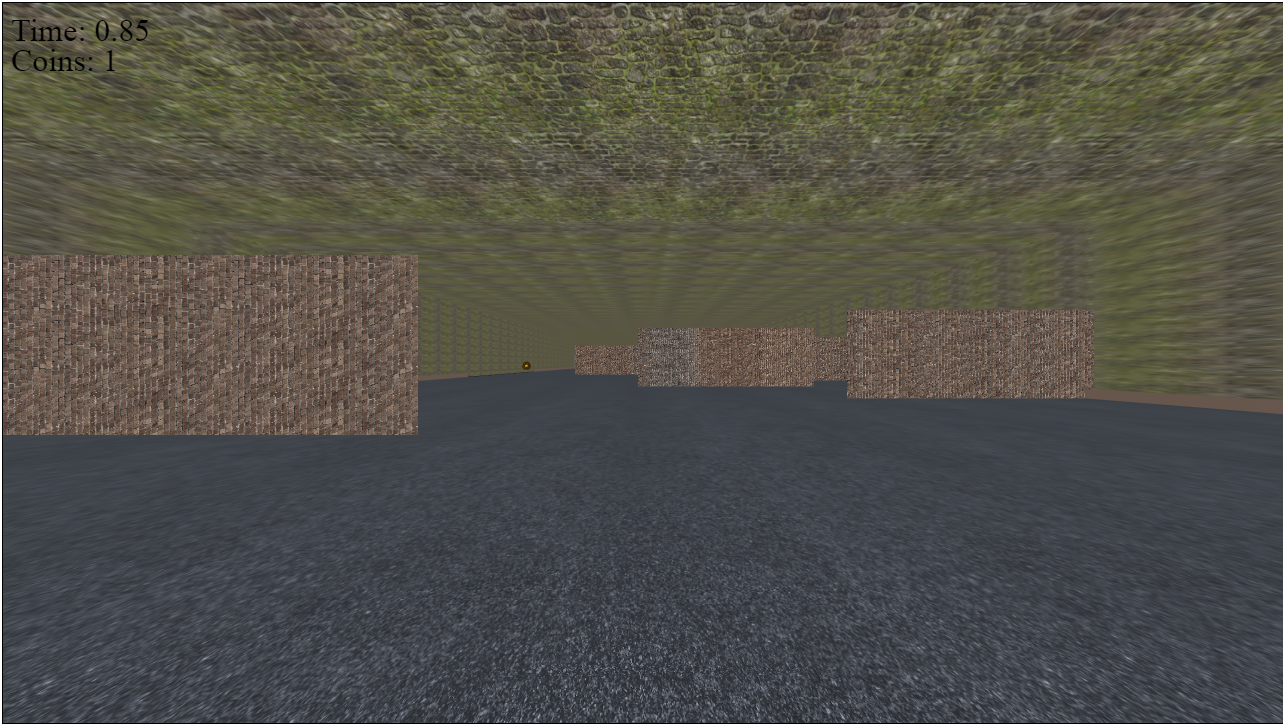
\includegraphics[width=\columnwidth]{gameplay.png}
		\caption{Igled igre} \label{fig:gameplay}
	\end{center}
\end{figure}
Odločila sva se da bova izdelala dirkaško igro\ref{fig:tunel}, katere je glavni namen izogibanje oviram, ter zaključiti progo z, čim več kovanci ter z daljšim časom saj čimveč kovancov kot jih pobereš dalj časa lahko igraš. Zahtevnost igre se povečuje na vsakih 20 procentov dolžine proge z povečanjem hitrosti prav tako za 20 procentov.
Igra je namenjena igralcem vseh starosti.
Igra se izvaja na ravni površini, katera je dolžine 900 (z: 0, z:900), ter širine 10 (x: -5,5). Objekti so v večini sestavljeni iz ravnih površin, razen kovanci kateri so krogi z robom 0.06.


\subsection{Opis sveta}
Na tem mestu podajte grob opis sveta v igri, ki ga podrobenje definirate v sledečih podpoglavjih. Prav tako definirajte v kakšnem stilu bo izdelan svet (npr. realističen, stiliziran, risankast, ipd.). Opredelite tudi ali se bodo osebki v svetu pomikali v eni, dveh ali treh dimenzijah.

\subsubsection{Pregled}

V najinem svetu sva naredila objekte s katerimi lahko interaktiramo. Ti objekti so na progi postavljeni naključno tako da se proga nikoli ne ponavlja. Tako je pa lahko tudi sama zahtevnost čisto naključna. Pri zidovih, če se igralec zaleti v njih, se odbije en kovanec in če je kovancev manj kot 1 je tako konec igre. Na progi imamo tudi kovance s katerimi lahko upočasnimo vozilo, ko naberemo 5 kovancev se nam hitrost pomanjša za 10 procentov. 

\subsubsection{Ozadje}
\begin{figure}[!htb]
	\begin{center}
		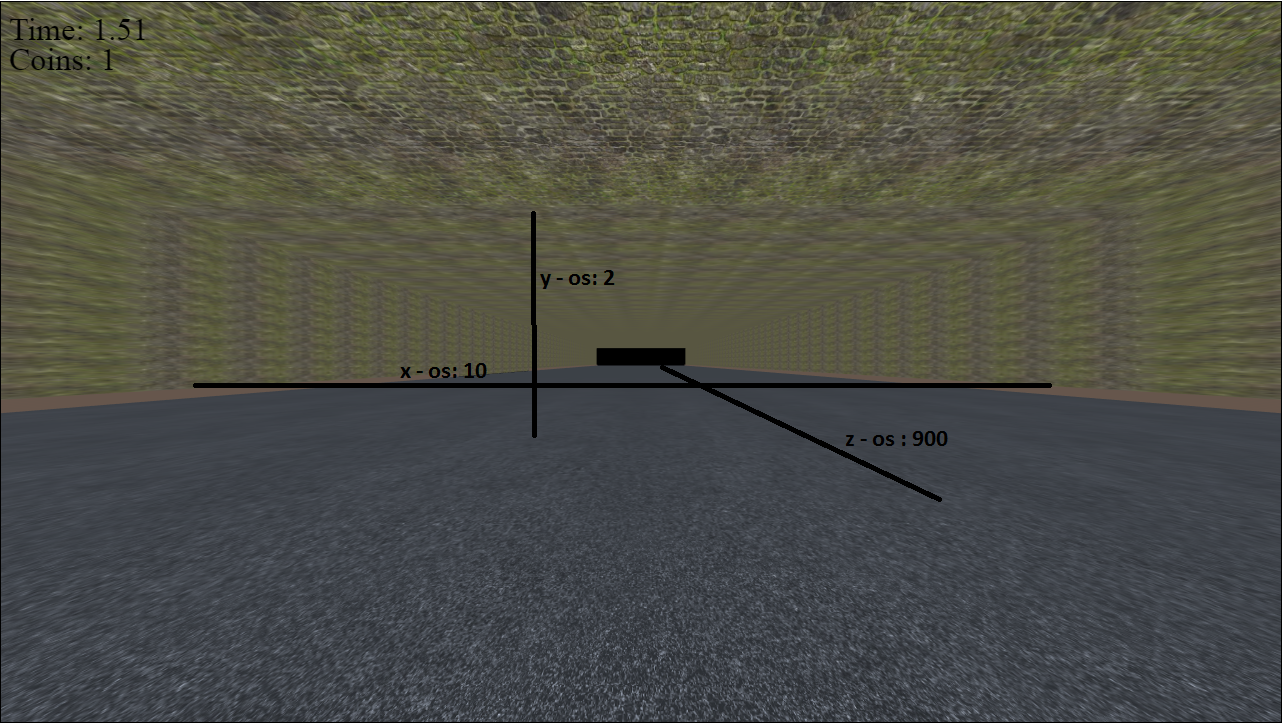
\includegraphics[width=\columnwidth]{tunel.png}
		\caption{Velikost tunela} \label{fig:tunel}
	\end{center}
\end{figure}
Igra se izvaja v tunelu\ref{fig:tunel}, v katerim ima uporabnik občutek »ujetosti«.  Strop ter stene so narejene iz opek, katere spominjajo na zelo staro gradnjo tunela. Robniki so pa zgrajeni iz rjavih opek. 


\subsubsection{Ključne lokacije}
Ključne lokacije so stene, robniki, zidovi, kovanci, ter vsaka petina proge. Stene so postavljene v svetu na točkah x:5.1 ter x:-5.1, robniki so postavljeni na x:5.0 ter x:-5.0, z robniki tudi vozilo iteratira, tako da nemore od te točke naprej po x-u. Zidovi ter kovanci so postavljeni v svet naključno po x osi, npr. zidovi se pojavijo vsakič ko se z os, poveča za 5. Kovanci pa ko se z os poveča za 18. Na vsaki petini proge pa se prav tako poveča hitrost. Ko pridemo do konca proge (z: 900), se igra konča z dialogom (»You won!«)

\subsubsection{Velikost}
Svet je predstavljen v tunelu, kateri je dimenzij 10x2x900 (x,y,z). Uporabnik pa interaktira samo po x osi.

\subsubsection{Objekti}
Celi svet sva izdelala sama, zidovi so izdelani iz dveh trikotniko kateri so širine 3. Kovanci so narejeni iz polmera 0.15 ter iz 100-ih trikotnikov, na ta trikotnik je še na oglišča poslavljen pravokotnih iz sosednjih oglišč tako dobimo zaobljen rob in celota spominja na kovanec. Stene, robniki, cesta so pa prav tako sestavljeni iz trikotnikom opisanih že v prejšnjih poglavjih.
\subsubsection{Čas}
Najina igra se odvija v realnem času.

\subsection{Igralni pogon in uporabljene tehnologije}
Za seminar sva uporabila WebGl\footnote{\url{https://webglfundamentals.org/}}\footnote{\url{https://web.archive.org/web/20171025022250/http://learningwebgl.com:80/blog/?page_id=1217}}, HTML, CSS, Javascript. Z HTML-jem, ter CSS-jem sva si pomagala za izpisovanje časa, ter števila kovancev na canvas, prav tako pa za uporabniški meni. Za Webgl nisva uporabila nobene dodatne knjižnice. Za trke sva sama spisala zaznavanje, naredila sva ovoj glede na širino objekta, s tem sva tudi določila mejo pri kateri se trk zazna. Pri trkih sva si tudi pomagala z časovno omejitvijo, tako da se lahko trk zgodi samo vsakih 200 milisekund. Isto zaznavanje sva uporabila tudi za to, da vozilo negre izven proge.

\subsection{Pogled}
Kamera je v prvi osebi in ima vidno polje 45 stopinj pred seboj. Vidi pred seboj od 0.1 pa do 950 enot.

\section{Osebek}
Uporabnik bo igral vozilo, v prvo osebnem pogledu. Vozilo bo lahko premikal z A ter D, ter z levo in desno smerno tipko. Osebek se stalno premika naprej po progi in se nemore ustavljati. Nad drugimi objekti nima nadzora.

\section{Uporabniški vmesnik}
Uporabniški vmesnik predstavi pravila igranja, ter začetek igre. Med igro je viden napis za čas ter stanje kovancev. Če zmanjka kovancev se tudi pojavi napis »Game over«, ter igra se postavi na začetni meni.Uporabniški vmesnik sva implementirala s pomočjo HTML-ja ter CSS-ja. Takšen vmesnik sva izbrala, ker je preprost dizajn in ne obremenjuje samo igro. 

\section{Glasba in zvok}
V igri je predstavljen samo zvok zagona motorja. Zvočni efekt sva pridobila z spletne strani freesoundeffect\footnote{\url{https://www.freesoundeffects.com/free-sounds/cars-10069/}}.

\section{Gameplay}
Igra se začne začne s pritiskom na »play« gumb. Začetna hitrost je nastavljena na 0.01, ta pa se tudi povečuje na vsako petino mape oziroma zniža za 10 procentov, če zberemo 5 kovančkev. Če jih toliko zberemo se tudi število kovancev zmanjša na 1, sepravi da smo relativno zmanjšali zahtevnost igre. Sam cilj igre je izogibanje ovir, ter varen prihod na cilj proge.


\section{Zaključki in možne nadgradnje}
Med samo izdelavo igre sva se naučila izdelovanje 3-d modelov, s pomočjo trikotnikov, delovanje filtrov na teksture, pri zaznavanju trkov. sva morala biti previdna na koliko časa bo program spet zaznač trk, tako sva tudi rešila problem na preprost način. Razlika med 



\small


\end{document}
